\chapter{Fundamentals} % Main chapter title

\label{Chapter2} % For referencing the chapter elsewhere, use \ref{Chapter2}
% TODO Sectionnamen: Die Namen der Sections sind nicht unbedingt sinnvoll und sind jetzt erstmal dazu da 
% mir selbst den Roten Faden aufzuzeigen
% \section{Virtual Memory}
% Grundlagen auffrischen, kurz die Motivation und Grundkonzepte von Virtual Memory erläutern
% Da eventuell kurz auf Atlas eingehen und wie sehr sich VM bis jetzt entwickelt hat
% Quellen:
% - Lehrbücher: VM Definitionen und Übersichtsbeschreibungen
% \subsection{What is Virtual Memory}


% Purpose of Section:
% Ziegen, dass es keinen Standard gibt und es viele Verschiedne Möglichkeiten gibt um VM zu realisieren
% Quellen:
% [ A look at several...]
% [ Issues of implementation]
% \section{Implementation of Virtual Memory Systems}
% \subsection{ Overview of different implementations (Inverted/Hierarchical/Multi-Level)}
% \subsection{ Comparison of differnt implementations with regards to performance and features like page sharing}

% \section{Hardware support}
% \subsection{MMU & TLB}
% \subsection{HW-Dependent PTE Structure}
% \subsection{A typical Page Table Walk}

% \section{ Sofware Paging approaches}
% \subsection{More flexibilty}

\begin{figure*}[t]
    \centering
    \begin{bytefield}[bitwidth=\widefigurewidth/39,bitheight=\widthof{~PBMT~}, bitformatting={\tiny\bfseries}, boxformatting={\centering}]{39}
        \bitheader[endianness=big]{38,30,29,21,20,12,11,0} \\
        \bitbox{9}{VPN[2]} &
        \bitbox{9}{VPN[1]} &
        \bitbox{9}{VPN[0]} &
        \bitbox{12}{Page Offset}\\
    \end{bytefield}
    \caption[RISC-V Sv39 Virtual Address]{RISC-V Sv39 Virtual Address}
    \label{fig:fundamentals:sv39va}
\end{figure*}

\begin{figure*}[t]
    \centering
    \begin{bytefield}[bitwidth=\widefigurewidth/56,bitheight=\widthof{~PBMT~}, bitformatting={\tiny\bfseries}, boxformatting={\centering}]{56}
        \bitheader[endianness=big]{55,30,29,21,20,12,11,0} \\
        \bitbox{26}{PPN[2]} &
        \bitbox{9}{PPN[1]} &
        \bitbox{9}{PPN[0]} &
        \bitbox{12}{Page Offset}\\
    \end{bytefield}
    \caption[RISC-V Sv39 Physical Address]{RISC-V Sv39 Physical Address}
    \label{fig:fundamentals:sv39pa}
\end{figure*}

\begin{figure*}[t]
    \centering
    \begin{bytefield}[bitwidth=\widefigurewidth/64,bitheight=\widthof{~PBMT~}, bitformatting={\tiny\bfseries}, boxformatting={\centering}]{64}
        \bitheader[endianness=big]{63,62,61,60,54,53,28,27,19,18,10,9,8,7,6,5,4,3,2,1,0} \\
        \bitbox{1}{N} &
        \bitbox{2}{\rotatebox{90}{PBMT}} &
        \bitbox{7}{Reserved} &
        \bitbox{26}{PPN[2]} &
        \bitbox{9}{PPN[1]} &
        \bitbox{9}{PPN[0]} &
        \bitbox{2}{\rotatebox{90}{RSW}} &
        \bitbox{1}{D} &
        \bitbox{1}{A} &
        \bitbox{1}{G} &
        \bitbox{1}{U} &
        \bitbox{1}{X} &
        \bitbox{1}{W} &
        \bitbox{1}{R} &
        \bitbox{1}{V}
    \end{bytefield}
    \caption[RISC-V Sv39 Page Table Entry]{RISC-V Sv39 Page Table Entry}
    \label{fig:fundamentals:sv39pte}
\end{figure*}
\begin{figure*}[t]
    \centering
    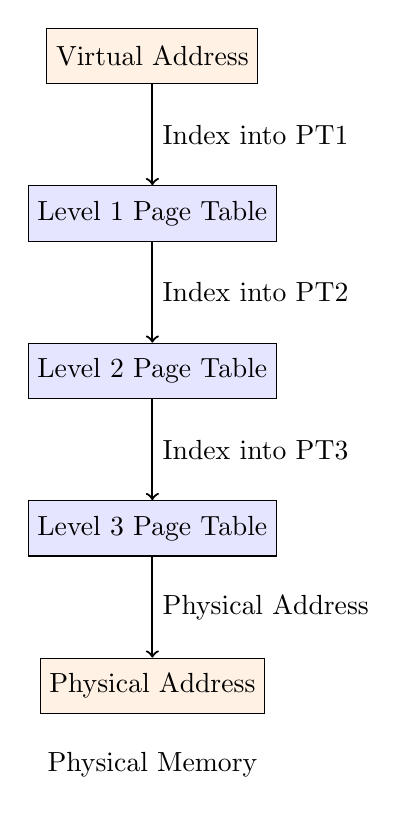
\begin{tikzpicture}[node distance=2cm, auto]
        % Define block styles
        \tikzstyle{pageTable} = [rectangle, draw, fill=blue!10, text centered, minimum height=2em, minimum width=4em]
        \tikzstyle{process} = [rectangle, draw, fill=orange!10, text centered, minimum height=2em, minimum width=6em]
        \tikzstyle{arrow} = [->, thick]

        % Nodes
        \node[process] (virtual) {Virtual Address};
        \node[pageTable, below of=virtual] (pt1) {Level 1 Page Table};
        \node[pageTable, below of=pt1] (pt2) {Level 2 Page Table};
        \node[pageTable, below of=pt2] (pt3) {Level 3 Page Table};
        \node[process, below of=pt3] (physical) {Physical Address};

        % Arrows
        \draw[arrow] (virtual) -- (pt1) node[midway, right] {Index into PT1};
        \draw[arrow] (pt1) -- (pt2) node[midway, right] {Index into PT2};
        \draw[arrow] (pt2) -- (pt3) node[midway, right] {Index into PT3};
        \draw[arrow] (pt3) -- (physical) node[midway, right] {Physical Address};

        % Optional: Add text labels or notes
        \node[below of=physical, node distance=1cm] {Physical Memory};

    \end{tikzpicture}

    \caption[RISC-V Sv39 Address Translation Process]{RISC-V Sv39 Address Translation Process}
    \label{fig:fundamentals:sv39addresstranslation}
\end{figure*}

\begin{tikzpicture}
    % Define styles
    \tikzstyle{section} = [draw, fill=blue!10, text centered, minimum height=2em, minimum width=4em]

    % Draw the main box
    \node[draw, rectangle, minimum width=6cm, minimum height=6cm] (mainbox) {};

    % Draw sections
    \node[section, below left=0.5cm and 0.5cm of mainbox.north west] (section1) {Section 1};
    \node[section, below right=0.5cm and 0.5cm of mainbox.north east] (section2) {Section 2};
    \node[section, below=1.5cm of section1.south] (section3) {Section 3};
    \node[section, below=1.5cm of section2.south] (section4) {Section 4};

    % Draw separating lines
    \draw[thick] (mainbox.west) -- (mainbox.east);
    \draw[thick] (section1.south west) -- (section2.south east);
    \draw[thick] (section3.west) -- (section4.east);
    \draw[thick] (section1.south west) -- (section3.north west);
    \draw[thick] (section2.south east) -- (section4.north east);

\end{tikzpicture}